\section{Introducing the Recycling folded-Cascode transcondutance amplifier}

This report was concieved about the study of a Recycling Folded Cascode (RFC) Operacional Transconductance Amplifier (OTA) circuit\textsuperscript{\cite{artigo-prof}}. The main goal of this study was to design and simulate a circuit, and observing the advantages of RFC OTA over the convencional Folded Cascode (FC) OTA. 

The circuit was designed using the TSMC 65nm technology and the design was done using the Cadence Virtuoso software. In Figure \ref{fig:OTA_schematic}is the schematic of the designed of the proposed circuit.

\begin{figure}[H]
    \centering
    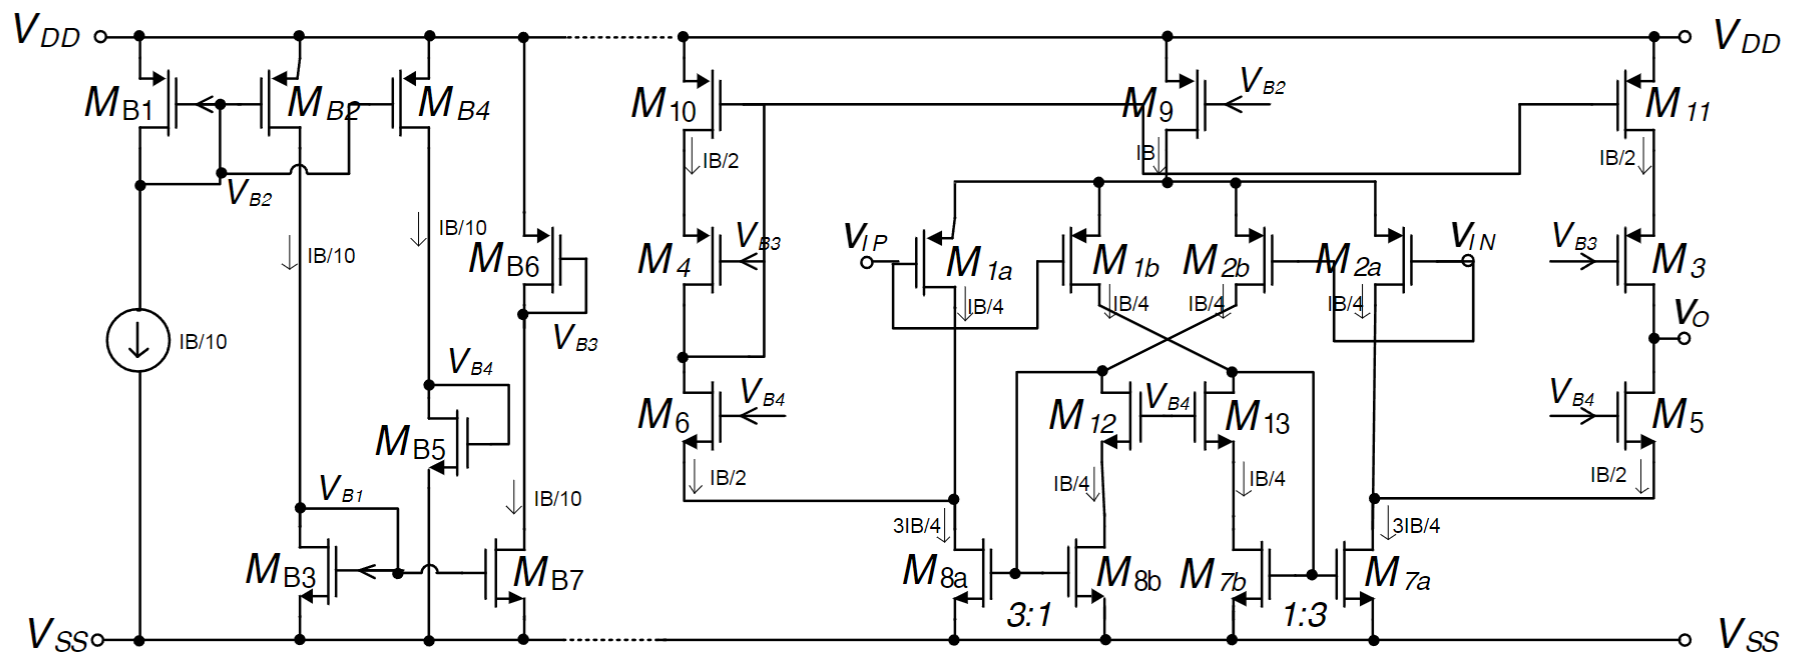
\includegraphics[width=1\textwidth]{Images/RFC_OTA_schematic.png}
    \caption{Recycling Folded Cascode OTA Schematic\textsuperscript{\cite{Lab-statement}}}
    \label{fig:OTA_schematic}
\end{figure}

The design was simulated and the results were analyzed and compared to the theoretical values. The results were then used to calculate the merit of the circuit.

\pagebreak

